\documentclass{beamer}

\mode<presentation> {

% The Beamer class comes with a number of default slide themes
% which change the colors and layouts of slides. Below this is a list
% of all the themes, uncomment each in turn to see what they look like.

%\usetheme{default}
%\usetheme{AnnArbor}
%\usetheme{Antibes}
%\usetheme{Bergen}
%\usetheme{Berkeley}
%\usetheme{Berlin}
%\usetheme{Boadilla}
%\usetheme{CambridgeUS}
%\usetheme{Copenhagen}
%\usetheme{Darmstadt}
%\usetheme{Dresden}
%\usetheme{Frankfurt}
%\usetheme{Goettingen}
%\usetheme{Hannover}
%\usetheme{Ilmenau}
%\usetheme{JuanLesPins}
%\usetheme{Luebeck}
\usetheme{Madrid}
%\usetheme{Malmoe}
%\usetheme{Marburg}
%\usetheme{Montpellier}
%\usetheme{PaloAlto}
%\usetheme{Pittsburgh}
%\usetheme{Rochester}
%\usetheme{Singapore}
%\usetheme{Szeged}
%\usetheme{Warsaw}

% As well as themes, the Beamer class has a number of color themes
% for any slide theme. Uncomment each of these in turn to see how it
% changes the colors of your current slide theme.

%\usecolortheme{albatross}
%\usecolortheme{beaver}
%\usecolortheme{beetle}
%\usecolortheme{crane}
%\usecolortheme{dolphin}
%\usecolortheme{dove}
%\usecolortheme{fly}
%\usecolortheme{lily}
%\usecolortheme{orchid}
%\usecolortheme{rose}
%\usecolortheme{seagull}
%\usecolortheme{seahorse}
%\usecolortheme{whale}
%\usecolortheme{wolverine}

%\setbeamertemplate{footline} % To remove the footer line in all slides uncomment this line
%\setbeamertemplate{footline}[page number] % To replace the footer line in all slides with a simple slide count uncomment this line

%\setbeamertemplate{navigation symbols}{} % To remove the navigation symbols from the bottom of all slides uncomment this line
}

\usepackage[utf8]{inputenc}
\usepackage[english]{babel}
% \usepackage[ngerman]{babel}

\usepackage{amsmath}
\usepackage{amssymb}
\usepackage{amsfonts}
\usepackage{xcolor}
\usepackage{graphicx}
\usepackage{float}
\usepackage{algorithm}
\usepackage[noend]{algpseudocode}

\let\oldReturn\Return
\renewcommand{\Return}{\State\oldReturn}

\definecolor{mygreen}{rgb}{0.01, 0.75, 0.24}

\usepackage{tikz}
\usetikzlibrary{arrows,decorations.pathmorphing,positioning,fit,trees,shapes,automata}
\usepackage{pgf-umlsd}
\usepgflibrary{arrows} % for pgf-umlsd

\tikzset{onslide/.code args={<#1>#2}{%
  \only<#1>{\pgfkeysalso{#2}} % \pgfkeysalso doesn't change the path
}}

\usepackage{listings}

%----------------------------------------------------------------------------------------
%	TITLE PAGE
%----------------------------------------------------------------------------------------

\title[Compositional safety verification]{On Compositional safety verification with Max-SMT} % The short title appears at the bottom of every slide, the full title is only on the title page

\author{Fabian B\"{o}ller with David Korzeniewski} % Your name
\institute[i2] % Your institution as it will appear on the bottom of every slide, may be shorthand to save space
{
RWTH Aachen \\ % Your institution for the title page
\medskip
\textit{fabian.boeller@rwth-aachen.de} % Your email address
}
\date{SS 2017} % Date, can be changed to a custom date

\begin{document}

\begin{frame}
\titlepage % Print the title page as the first slide
\end{frame}

\begin{frame}
\frametitle{Overview} % Table of contents slide, comment this block out to remove it
\tableofcontents % Throughout your presentation, if you choose to use \section{} and \subsection{} commands, these will automatically be printed on this slide as an overview of your presentation
\end{frame}

%----------------------------------------------------------------------------------------
%	PRESENTATION SLIDES
%----------------------------------------------------------------------------------------

\section{Introduction}

\begin{frame}
  \frametitle{Terms}
  \begin{block}{Safety verification}
    Prove that an assertion is \emph{always} true at a location
  \end{block}
  \pause
  \begin{block}{Non-compositional safety verification}
    Safety verification where the whole program is analyzed in one step
  \end{block}
  \pause
  \begin{block}{Compositional safety verification}
    Safety verification where program parts are analyzed semi-independently and composed
  \end{block}
\end{frame}

\begin{frame}
  \frametitle{Motivation}
  \begin{figure}
    \centering
    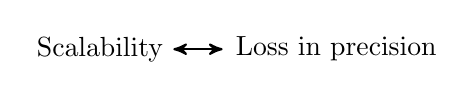
\begin{tikzpicture}[->,>=stealth',shorten >=1pt,auto,node distance=3cm,thick]
      \node (1) {Scalability};
      \node (2) [right of=1] {Loss in precision};
      \path[<->]
      (1) edge node {} (2);
    \end{tikzpicture}
  \end{figure}
\end{frame}

\section{Program graphs}

\begin{frame}[t]
  \frametitle{Programs}
  \begin{block}{Program}
    $\mathcal{L} = \lbrace \ell_0, \ell_1, \ell_2 \rbrace$
    \only<2->{, $\mathcal{T} = \lbrace t_i \mid i \in \lbrace 1,\dots,6 \rbrace \rbrace$}
    \only<3->{, $\mathcal{V} = \lbrace x,y,i \rbrace$, $\mathcal{V}' = \lbrace x',y',i' \rbrace$}
  \end{block}
  \begin{overlayarea}{\linewidth}{\textheight}
  \begin{figure}
    \centering
    \begin{tikzpicture}[->,>=stealth',auto,node distance=3cm,
        thick,
        main node/.style={circle,draw,font=\sffamily\Large\bfseries},
        aligned edge/.style={align=left},
        scc0/.style={draw=orange, text=orange},
        scc1/.style={draw=mygreen, text=mygreen},
        scc2/.style={draw=blue, text=blue},
        new/.style={draw=blue, text=blue},
        newtext/.style={text=blue}]

      \node[main node, onslide={<1>new}, onslide={<5->scc0}] (0) {$l_0$};
      \node[main node, onslide={<1>new}, onslide={<5->scc1}] (1) [right of=0] {$l_1$};
      \node[main node, onslide={<1>new}, onslide={<5->scc2}] (2) [right of=1] {$l_2$};
      
      \node (4) [right of=2] {};
      \node (5) [left of=0] {};

      \onslide<2->{
        \path[every node/.style={font=\sffamily\small}]
        (0) edge[aligned edge, onslide={<2>new}] node {$t_1$\only<3->{$: $ \only<3>{\color{blue}} $x \geq y$}} (1)
        (0) edge[aligned edge, onslide={<2>new}, bend right=25] node [below] {$t_2$\only<3->{$: $\only<3>{\color{blue}} $y > x$}} (2)
        (1) edge[aligned edge, onslide={<2>new}, loop above, onslide={<5->scc1}] node {$t_3$\only<3->{$: $\\ \only<3>{\color{blue}} $i > 0 \wedge$\\ \only<3>{\color{blue}} $x' = x + 1 \wedge$\\ \only<3>{\color{blue}} $i' = i - 1$}} (1)
        (1) edge[aligned edge, onslide={<2>new}] node {$t_4$\only<3->{$: $ \only<3>{\color{blue}} $i = 0$}} (2)
        (2) edge[aligned edge, onslide={<2>new}, loop above, onslide={<5->scc2}] node {$t_5$\only<3->{$: $\\ \only<3>{\color{blue}} $x' = x + 1 \wedge$\\ \only<3>{\color{blue}} $y' = y + 1$}} (2)
        (2) edge[aligned edge, onslide={<2>new}] node {$t_6$\only<4->{\only<4>{\color{blue}}, assert($x \neq y$)}} (4)
        (5) edge[aligned edge, onslide={<2>new}] node {$t_0$\only<3->{$: $ \only<3>{\color{blue}} $i > 0$}} (0);
      }
    \end{tikzpicture}
  \end{figure}
  \end{overlayarea}
\end{frame}

\section{Algorithm overview}

\begin{frame}
  \frametitle{CheckSafe}
  \begin{block}{Idea}
    Prove that an assertion is satisfied by recursively checking all entry components
  \end{block}
  \begin{figure}
    \centering
    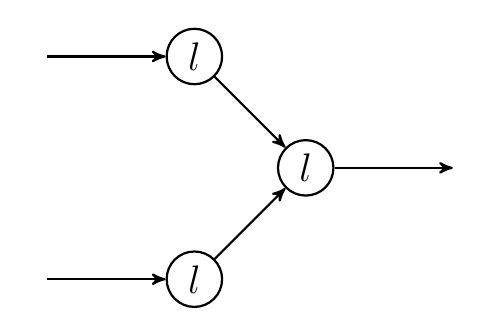
\begin{tikzpicture}[->,>=stealth',auto,node distance=2cm,
        thick,
        main node/.style={circle,draw,font=\sffamily\Large\bfseries},
        inspect/.style={draw=blue, text=blue},
        safe/.style={draw=mygreen, text=mygreen},
        maybe/.style={draw=orange, text=orange},
        changed/.style={ultra thick},
        aligned edge/.style={align=left}]

      \node[main node,
        onslide={<2->inspect}, onslide={<2>changed},
        onslide={<11>safe}, onslide={<11>changed}
      ] (0) {$l$};
      \node[main node,
        onslide={<3-5>inspect}, onslide={<3>changed},
        onslide={<6->safe}, onslide={<6>changed}
      ] (1) [above left of=0] {$l$};
      \node[main node,
        onslide={<7-9>inspect}, onslide={<7>changed},
        onslide={<10->safe}, onslide={<10>changed}
      ] (2) [below left of=0] {$l$};
      
      \node (11) [left of=1] {};
      \node (21) [left of=2] {};
      \node (exit) [right of=0] {};

      \path[every node/.style={font=\sffamily\small}]
      (1) edge[
        onslide={<3-5>inspect}, onslide={<3>changed},
        onslide={<6->safe}, onslide={<6>changed}
      ] node {} (0)
      (2) edge[
        onslide={<7-9>inspect}, onslide={<7>changed},
        onslide={<10->safe}, onslide={<10>changed}
      ] node {} (0)
      (11) edge[
        onslide={<4>inspect}, onslide={<4>changed},
        onslide={<5->safe}, onslide={<5>changed}
      ] node {} (1)
      (21) edge[
        onslide={<8>inspect}, onslide={<8>changed},
        onslide={<9->safe}, onslide={<9>changed}
      ] node {} (2)
      (0) edge[
        onslide={<2-10>inspect}, onslide={<2>changed},
        onslide={<11>safe}, onslide={<11>changed}
      ] node {} (exit);
    \end{tikzpicture}
  \end{figure}
\end{frame}

\begin{frame}
  \frametitle{CondSafe}
  \begin{block}{Idea}
    Find a precondition for a component such that all runs satisfying the precondition always imply the postcondition
  \end{block}
  \begin{figure}
    \centering
    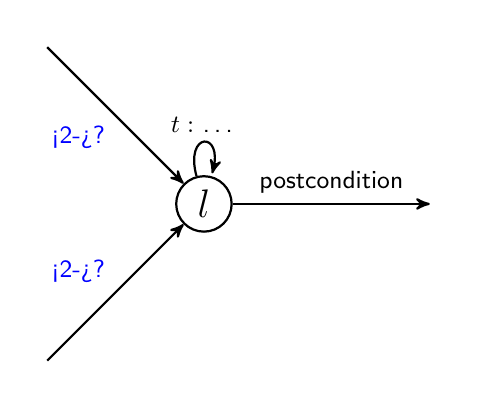
\begin{tikzpicture}[->,>=stealth',auto,node distance=3cm,
        thick,
        main node/.style={circle,draw,font=\sffamily\Large\bfseries},
        aligned edge/.style={align=left}]

      \node[main node] (0) {$l$};
      
      \node (1) [above left of=0] {};
      \node (2) [below left of=0] {};
      \node (exit) [right of=0] {};

      \path[every node/.style={font=\sffamily\small}]
        (1) edge[text=blue] node[below left] {\only<2->{?}} (0)
        (2) edge[text=blue] node[above left] {\only<2->{?}} (0)
        (0) edge[aligned edge, loop above] node {$t: $ \dots} (0)
        (0) edge node {postcondition} (exit);
    \end{tikzpicture}
  \end{figure}
\end{frame}

\begin{frame}
  \frametitle{Narrowing}
  \begin{block}{Idea}
    Manipulate the program such that new preconditions can be found
  \end{block}
  \begin{figure}
    \centering
    \begin{tikzpicture}[->,>=stealth',auto,node distance=2.5cm,
        thick,
        main node/.style={circle,draw,font=\sffamily\Large\bfseries},
        inspect/.style={draw=blue, text=blue},
        safe/.style={draw=mygreen, text=mygreen},
        maybe/.style={draw=orange, text=orange},
        aligned edge/.style={align=left}]

      \node[main node, onslide={<1-3>inspect}, onslide={<4>safe}] (0) {$l$};
      \node[main node, onslide={<1->safe}] (1) [above left of=0] {$l$};
      \node[main node, onslide={<1>maybe}, onslide={<2>inspect}, onslide={<3->safe}] (2) [below left of=0] {$l$};
      
      \node (11) [left of=1] {};
      \node (21) [left of=2] {};
      \node (exit) [right of=0] {};

      \path[every node/.style={font=\sffamily\small}]
        (0) edge[aligned edge, loop above, onslide={<1-3>inspect}, onslide={<4>safe}] node {$t_0: \varphi_0$\only<2->{\\$\wedge \dots$}} (0)
        (1) edge[aligned edge, onslide={<1->safe}] node [below left] {$t_1: \varphi_1$\only<2->{\\$\wedge \dots$}} (0)
        (2) edge[aligned edge, onslide={<1>maybe}, onslide={<2>inspect}, onslide={<3->safe}] node {$t_2: \varphi_2$\only<2->{\\$\wedge \dots$}} (0)
        (11) edge[onslide={<1->safe}] node {} (1)
        (21) edge[onslide={<1>maybe}, onslide={<2>inspect}, onslide={<3->safe}] node {} (2)
        (0) edge[onslide={<1-3>inspect}, onslide={<4>safe}] node {} (exit);
    \end{tikzpicture}
  \end{figure}
\end{frame}

\section{Example execution}

\begin{frame}
  \frametitle{Example program}
  \begin{figure}
    \centering
    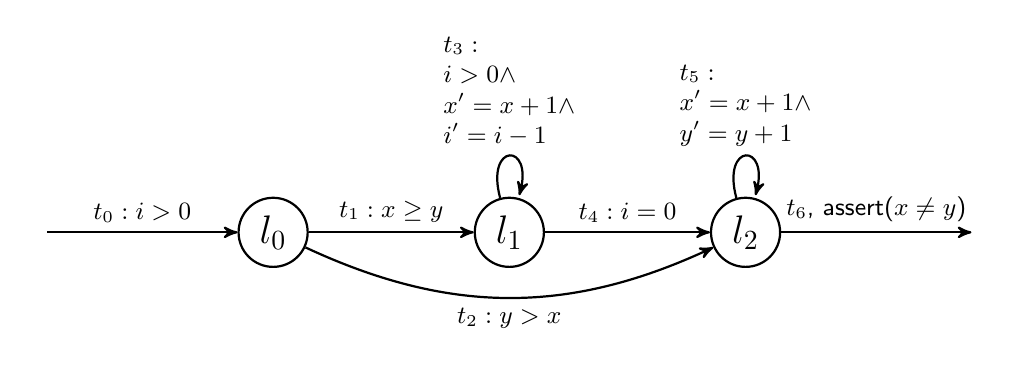
\begin{tikzpicture}[->,>=stealth',auto,node distance=3cm,
        thick,
        main node/.style={circle,draw,font=\sffamily\Large\bfseries},
        aligned edge/.style={align=left}]
      
      \node[main node] (0) {$l_0$};
      \node[main node] (1) [right of=0] {$l_1$};
      \node[main node] (2) [right of=1] {$l_2$};
      
      \node (4) [right of=2] {};
      \node (5) [left of=0] {};
      
      \path[every node/.style={font=\sffamily\small}]
      (0) edge[aligned edge] node {$t_1: x \geq y$} (1)
      edge[aligned edge, bend right=25] node [below] {$t_2: y > x$} (2)
      (1) edge[aligned edge, loop above] node {$t_3:$\\$i > 0 \wedge$\\$x' = x + 1 \wedge$\\$i' = i - 1$} (1)
      edge[aligned edge] node {$t_4: i = 0$} (2)
      (2) edge[aligned edge, loop above] node {$t_5:$\\$x' = x + 1 \wedge$\\$y' = y + 1$} (2)
      edge[aligned edge] node {$t_6$, assert($x \neq y$)} (4)
      (5) edge[aligned edge] node {$t_0: i > 0$} (0);
    \end{tikzpicture}
  \end{figure}
\end{frame}

\begin{frame}
  \frametitle{Example execution}
  \begin{figure}
    \centering
    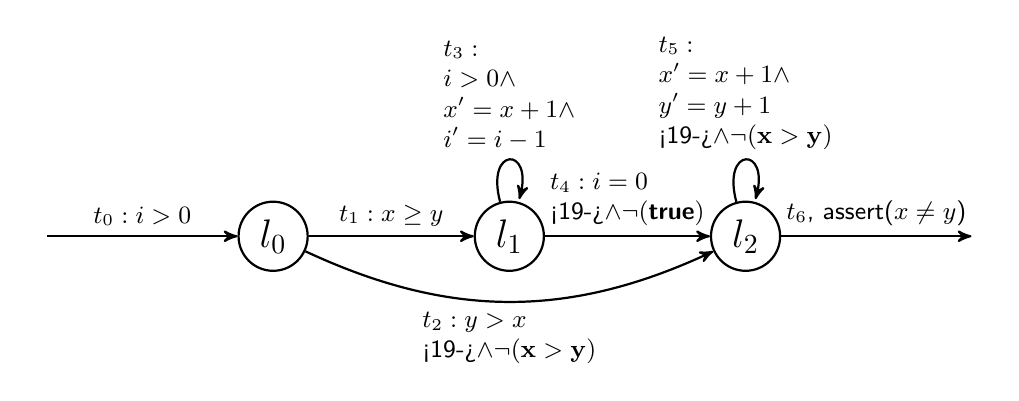
\begin{tikzpicture}[->,>=stealth',auto,node distance=3cm,
        thick,
        main node/.style={circle,draw,font=\sffamily\Large\bfseries},
        aligned edge/.style={align=left},
        inspect/.style={draw=blue, text=blue},
        safe/.style={draw=mygreen, text=mygreen},
        maybe/.style={draw=orange, text=orange},
        maxsmt/.style={draw=red, text=red},
        changed/.style={ultra thick}
      ]
      
      \node[main node, onslide={<9>inspect}, onslide={<12-14>inspect}, onslide={<15>safe}, onslide={<16>inspect}, onslide={<17>safe}, onslide={<21>inspect}] (0) {$l_0$};
      \node[main node, onslide={<11-17>inspect}, onslide={<18>safe}] (1) [right of=0] {$l_1$};
      \node[main node, onslide={<2-22>inspect}, onslide={<23>safe}] (2) [right of=1] {$l_2$};
      
      \node (4) [right of=2] {};
      \node (5) [left of=0] {};
      
      \path[every node/.style={font=\sffamily\small}]
      (0)
      edge [aligned edge,
        onslide={<12>changed}, onslide={<12-14>inspect},
        onslide={<15>changed}, onslide={<15>safe},
        onslide={<16>changed}, onslide={<16>inspect},
        onslide={<17>changed}, onslide={<17>safe}]
      node {$t_1: x \geq y$}
      (1)

      (0)
      edge [aligned edge, bend right=25,
        onslide={<4,8>changed}, onslide={<4,8>maxsmt},
        onslide={<9>changed}, onslide={<9>inspect},
        onslide={<10>changed}, onslide={<10-18>maybe},
        onslide={<21>changed}, onslide={<21>inspect},
        onslide={<22>changed}, onslide={<22>safe},
        onslide={<19>changed}]
      node [below] {$t_2: y > x$\\\only<19->{$\wedge \mathbf{\neg (x > y)}$}}
      (2)

      (1)
      edge [aligned edge, loop above,
        onslide={<11>changed}, onslide={<11-16>inspect},
        onslide={<18>changed}, onslide={<18>safe}]
      node {$t_3:$\\$i > 0 \wedge$\\$x' = x + 1 \wedge$\\$i' = i - 1$}
      (1)

      (1)
      edge [aligned edge,
        onslide={<5,8>changed}, onslide={<5,8>maxsmt},
        onslide={<11>changed}, onslide={<11-17>inspect},
        onslide={<18>changed}, onslide={<18>safe},
        onslide={<21>changed}, onslide={<21>inspect},
        onslide={<22>changed}, onslide={<22>safe},
        onslide={<19>changed}]
      node {$t_4: i = 0$\\\only<19->{$\wedge \mathbf{\neg (\textbf{true})}$}}
      (2)

      (2)
      edge [aligned edge, loop above,
        onslide={<2>changed}, onslide={<2-5,7,9-22>inspect},
        onslide={<6,8>changed}, onslide={<6,8>maxsmt},
        onslide={<23>changed}, onslide={<23>safe},
        onslide={<19>changed}]
      node {$t_5:$\\$x' = x + 1 \wedge$\\$y' = y + 1$\\\only<19->{$\wedge \mathbf{\neg (x > y)}$}}
      (2)

      (2)
      edge [aligned edge,
        onslide={<1>changed}, onslide={<1-6,9-22>inspect},
        onslide={<7,8>changed}, onslide={<7,8>maxsmt},
        onslide={<23>changed}, onslide={<23>safe}]
      node {$t_6$, assert($x \neq y$)}
      (4)

      (5)
      edge[aligned edge,
        onslide={<13>changed}, onslide={<13>inspect},
        onslide={<14>changed}, onslide={<14>safe}]
      node {$t_0: i > 0$}
      (0);
    \end{tikzpicture}
  \end{figure}

  \only<1>{
    \begin{block}{Task}
      Prove that the program is safe for $x \neq y$ at $t_6$
    \end{block}
  }

  \only<2>{
    \begin{block}{CheckSafe on $\lbrace \ell_2 \rbrace$ for $x \neq y$}
      $t_6$ does not already imply $x \neq y$\\
      $t_6$ is not an initial transition\\
      Call CondSafe
    \end{block}    
  }

  \only<3-8>{
    \begin{block}{Max-SMT on $\lbrace \ell_2 \rbrace$ for $x \neq y$}
      \only<3>{$I_{\ell_2,1}(\lbrace x, y, i \rbrace) \equiv i_{\ell_2,1} + i_{\ell_2,1,x} * $ \textcolor{red}{x} $ + i_{\ell_2,1,y} * $ \textcolor{red}{y} $ + i_{\ell_2,1,i} * $ \textcolor{red}{i} $ \leq 0$}
      \only<4>{$\mathbb{I}_{t_2, 1, 1} \equiv $ \textcolor{red}{$y > x \wedge i' = i \wedge x' = x \wedge y' = y$} $\Rightarrow I'_{\ell_2,1,1}$}
      \only<5>{$\mathbb{I}_{t_4, 1, 1} \equiv $ \textcolor{red}{$i = 0 \wedge i' = i \wedge x' = x \wedge y' = y$} $\Rightarrow I'_{\ell_2,1,1}$}
      \only<6>{$\mathbb{C}_{t_5, 1} \equiv I_{\ell_2,1} \wedge $ \textcolor{red}{$x' = x + 1 \wedge y' = y + 1 \wedge i' = i$} $\Rightarrow I'_{\ell_2,1}$}
      \only<7>{$\mathbb{S}_1 \equiv I_{\ell_2,1} \wedge $ \textcolor{red}{$i' = i \wedge x' = x \wedge y' = y$} $\Rightarrow x' \neq y'$}
      \only<8>{
        $\mathbb{F}_1 \equiv \mathbb{C}_{t_5, 1} \wedge \mathbb{S}_1 \wedge (\mathbb{I}_{t_2,1,1} \vee \neg p_{t_2}) \wedge (\mathbb{I}_{t_4,1,1} \vee \neg p_{t_4}) \wedge [p_{t_2}, 1] \wedge [p_{t_4}, 1]$\\
        Assume $x > y$ does satisfy $\mathbb{F}_1$
      }
    \end{block}
  }

  \begin{overlayarea}{\linewidth}{\textheight}
  
  \only<9>{
    \begin{block}{CheckSafe on $\lbrace \ell_0 \rbrace$ for $x > y$}
      $t_2$ does not already imply $x > y$\\
      $t_2$ is not an initial transition\\
      Call CondSafe
    \end{block}    
  }

  \only<10>{
    \begin{block}{CheckSafe on $\lbrace \ell_0 \rbrace$ for $x > y$}
      No precondition, since $y > x$ contradicts $x > y$\\
      Path is maybe safe, but not for $x > y$
    \end{block}    
  }

  \only<11>{
    \begin{block}{CheckSafe on $\lbrace \ell_1 \rbrace$ for $x > y$}
      $t_4$ does not already imply $x > y$\\
      $t_4$ is not an initial transition\\
      Call CondSafe, get $i > 0 \wedge x \geq y$ as precondition
    \end{block}    
  }

  \only<12>{
    \begin{block}{CheckSafe on $\lbrace \ell_0 \rbrace$ for $i > 0$}
      $t_1$ does not already imply $i > 0$\\
      $t_1$ is not an initial transition\\
      Call CondSafe, get $i > 0$ as precondition
    \end{block}    
  }

  \only<13>{
    \begin{block}{CheckSafe on initial SCC for $i > 0$}
      $t_0$ does already imply $i > 0$
    \end{block}    
  }

  \only<14>{
    \begin{block}{CheckSafe on initial SCC for $i > 0$}
      Path is safe for $i > 0$
    \end{block}    
  }

  \only<15>{
    \begin{block}{CheckSafe on $\lbrace \ell_0 \rbrace$ for $i > 0$}
      Path is safe for $i > 0$
    \end{block}    
  }

  \only<16>{
    \begin{block}{CheckSafe on $\lbrace \ell_0 \rbrace$ for $x \geq y$}
      $t_1$ does already imply $x \geq y$
    \end{block}    
  }

  \only<17>{
    \begin{block}{CheckSafe on $\lbrace \ell_0 \rbrace$ for $x \geq y$}
      Path is safe for $x \geq y$
    \end{block}    
  }

  \only<18>{
    \begin{block}{CheckSafe on $\lbrace \ell_1 \rbrace$ for $x > y$}
      Path is safe for $x > y$
    \end{block}    
  }

  \only<19>{
    \begin{block}{Narrow on $\lbrace \ell_2 \rbrace$}
      Add $\neg (x > y)$ to $t_2$\\
      Add $\neg (x > y)$ to $t_5$
    \end{block}    
  }

  \only<20>{
    \begin{block}{CheckSafe on $\lbrace \ell_2 \rbrace$ for $x \neq y$}
      Call CondSafe, get $y > x$ instead of $x > y$ as precondition
    \end{block}    
  }

  \only<21>{
    \begin{block}{CheckSafe on $\lbrace \ell_0 \rbrace$ for $y > x$}
      $t_2$ does already imply $y > x$
      $t_4$ does already imply $y > x$
    \end{block}    
  }

  \only<22>{
    \begin{block}{CheckSafe on $\lbrace \ell_0 \rbrace$ for $y > x$}
      Paths are safe for $y > x$
    \end{block}    
  }

  \only<23>{
    \begin{block}{CheckSafe on $\lbrace \ell_0 \rbrace$ for $y > x$}
      Program is safe for $x \neq y$
    \end{block}    
  }

  \end{overlayarea}
  
\end{frame}

\section{Conclusion}

\begin{frame}
  \frametitle{Conclusion}
  \begin{block}{We saw:}
    \begin{enumerate}
    \item The exploration of multiple entry SCCs by CheckSafe
    \item The effect of narrowing if a path to the SCC is proved safe and another could not be proved safe
    \item The behavior of CheckSafe if a precondition with multiple conjunctions is found
    \end{enumerate}
  \end{block}
  \begin{block}{We didn't saw:}
    \begin{enumerate}
    \item SCCs with multiple transitions (effects consecution conditions in Max-SMT and entry locations in Narrowing)
    \end{enumerate}
  \end{block}
\end{frame}


\end{document} 
